\documentclass[openany, oneside, a4paper, 12pt, final]{memoir}
\usepackage{fontspec}
\usepackage[hidelinks]{hyperref}
\usepackage[natbib=true, style=numeric, backend=biber, sorting=none]{biblatex}
\usepackage{caption}
\usepackage[czech]{babel}
\usepackage[final]{microtype}
\addbibresource[datatype=bibtex]{vcely.bib}
\usepackage{booktabs}
\usepackage{graphicx}
\usepackage{siunitx}
\setmainfont{TeX Gyre Pagella}
\usepackage{xcolor}
\hypersetup{
	pdfauthor={MVDr. Magdaléna Pečinková},
	pdftitle={Otravy včel rostlinami},
	pdfkeywords={včela, toxin, otrava, rostliny},
	colorlinks,
	linkcolor={red!50!black},
	citecolor={blue!50!black},
	urlcolor={blue!80!black}
}
\setlrmarginsandblock{3.5cm}{2.5cm}{*}
\setulmarginsandblock{2.5cm}{*}{1}
\checkandfixthelayout
\addtopsmarks{headings}{}{ 
	\createmark{chapter}{left}{shownumber}{}{. \ } 
} 
\pagestyle{headings}

\sisetup{output-decimal-marker={,}}


\newcommand{\todo}[1]{{\color{purple} #1}}

\renewcommand{\printchaptername}{}

\title{Otravy včel rostlinami}
\author{Magdaléna Pečinková\\ AF MENDELU v Brně\\ 1. ročník - Všeobecné zemědělství K \\ Včelařství K}
\date{LS 2020}

\begin{document}
\frontmatter
\pagestyle{empty}
\maketitle
\clearpage
\tableofcontents
\mainmatter
\chapter*{Úvod}
\label{chap:intro}
\addcontentsline{toc}{chapter}{\nameref{chap:intro}}
Otravy včel mohou způsobit závažné ztráty a hynutí včel a včelstev. Může se jednat o otravy přirozené i umělé, vzniklé nedbalostí nebo nesprávným použitím chemických prostředků i o otravy úmyslné. Nejzávažnější jsou však otravy vyvolané použitím různých pesticidních prostředků v zemědělství. Nejnebezpečnější jsou především insekticidy, případně akaricidy s insekticidními účinky.  \cite{Multimedpomucka, vcelarstviVeselý, svobodovaveterinarni} 

Další ztráty včel mohou být způsobeny toxickými rostlinami, kterým se věnuje tato seminární práce. Text obsahuje obecný úvod do otrav včel, jejich diagnostiku, řešení i legislativní podklad. Druhá část je věnována konkrétním přírodním toxikantům vyskytujícím se na našem území i na jiných kontinentech, které byly analyzovány v několika odborných studiích.

\chapter{Otravy včel}
Ve včelstvu se denně líhne několik set až tisíc dělnic, mírnou chemickou otravu proto včelstvo během několika dnů zvládne překonat. Významnou vlastností včel je jejich společenský způsob života ve včelstvech, jehož důležitou součástí je vzájemné předávání potravy trofolaxí. Společně s potravou si však předávají jak léčiva, tak i toxické látky. Z~toho důvodu působí největší škody toxikanty s dlouhou reziduální dobou účinnosti (působící pomalu), která umožňuje kontaminaci velkého počtu včel ve včelstvu. Létavky po jejich požití nehynou okamžitě, ale vrátí se do úlu a v přinesené potravě předají toxickou látku dalším včelám. \cite{vcelarstviVeselý, svobodovaveterinarni}

Nejvýraznějším klinickým příznakem je hynutí včel, ke kterému může docházet přímo na porostech nebo v jejich blízkosti, případně na letové dráze k~úlům. V případě zanesení toxické látky do úlů může docházet i k úhynu úlových včel, případně plodu. Postižené včely se mohou shromažďovat i na česně, před úlem i na dně úlu. Může dojít i k ucpání česna a zapaření a udušení hynoucích včel. Uhynulé včely mohou být ulepené od vyvrhnutého obsahu medného váčku.

Diagnóza se stanoví na základě anamnestických údajů, klinických příznaků, patologických změn a toxikologického vyšetření. K chromatografickému průkazu toxické látky se odebírá vzorek nejméně 500~kusů včel (cca 60~g) a v případě podezření na otravu pesticidy nejméně 200~g ošetřovaného porostu. \cite{vyhlaska327} V~případě potřeby je možné odebrat i plásty s podezřelým pylem nebo medem. Při úhynu plodu i plodové plásty. 

Prevence u přirozených toxikóz spočívá v neumísťování úlů v blízkosti zdrojů toxického nektaru, pylu či medovice, u průmyslových otrav pak především v omezení chovu v blízkosti průmyslových závodů. Pro prevenci otrav léčivy je třeba dodržovat přesně návod na použití a dávkování. V případě otrav pesticidními prostředky je třeba dodržovat zásady ochrany včel vycházející ze zákona o rostlinolékařské péči (č. 326/2004 Sb.) a vyhlášky o ochraně včel, zvěře, vodních organismů a dalších organismů při použití přípravků na ochranu rostlin (č. 327/2012 Sb.), ve znění pozdějších předpisů. Jde především o to, neaplikovat zvláště nebezpečné přípravky na kvetoucí porosty (na 1~m\textsuperscript{2} kvetou více jak 2 rostliny), přípravky nebezpečné aplikovat až po skočení letu včel (denní let včel je ukončen hodinu po západu slunce), ale nejpozději do 23:00~hod. Důležitým preventivním opatřením je nahlášení stanovišť na obecní úřady (dané Plemenářským zákonem a Vyhláškou č.~136/2004 Sb.). \cite{Multimedpomucka, vyhlaska327} 

\chapter{Otravy včel rostlinami}

Odedávna včely přicházejí do styku s přírodními toxikanty z nektaru, medovice a~pylu rostlin, kde mívají povahu hlavně alkaloidů, glykosidů, nebo jednoduchých cukrů. Některé přírodní toxiny mohou být včelami velmi dobře snášeny, zatímco ve vysokých koncentracích mohou způsobovat otravy. V podmínkách střední Evropy však přírodní rostlinné toxiny nepředstavují pro včely vážné nebezpečí. Pokud~bychom se podívali za hranice České republiky, rostlin toxických pro včely bychom našli poměrně více. 
~\cite{svobodovaveterinarni,johnson2015honey}

Problém by mohl nastat pouze v místech rozsáhlého rozšíření toxické rostliny. U včel pozorujeme ojedinělou vlastnost tzv. florokonstantnost, tj. věrnost jednomu druhu květů -- nikdy nenavštěvují dva či více druhů rostlin v jednu dobu. Pokud jsou v~blízkosti dva druhy rostlin, které mají velké množství nektaru v jinou denní dobu, je možné, že včela bude navštěvovat oba (např. jeden ráno, druhý k večeru). \cite{Pridal} Pokud budou včely létat na jeden druh rostliny, která je pro ně toxická, může dojít k velkým ztrátám ve včelstvu. Pokud mají větší výběr kvetoucích rostlin, květům s toxickým nektarem se naučí poměrně rychle vyhýbat. \cite{pain2015sweet}


\section{Přírodní toxikanty}
Rostliny obsahují toxické sloučeniny hlavně jako ochranu před býložravci nebo mikroorganismy. Proto není překvapivé, že jsou obsaženy i v pylu a nektaru, tj. blízko reprodukčních orgánů, ačkoliv jejich největší koncentrace bývá v listech, prašnících a květech.

\subsection{Rostliny netoxické pro včely}
Známe řadu toxických rostlin, které však nemají toxický nektar ani pyl. Mezi takové rostliny patří například blín (\textit{Hyoscyamus niger}), rozpuk (\textit{Cicuta virosa}) nebo náprstník (\textit{Digitalis purpurea}).


Zároveň existují rostliny netoxické pro včely, jejichž toxické složky se dostávají do~medu a tím jsou nebezpečné pro zdraví člověka. Popisované jsou jedovaté medy z rododendronů (\textit{Andromeda}) obsahující gryanotoxin (též známý jako andromedotoxin) způsobující ochrnutí končetin až smrt. Dále pak medy z rostlin rodu \textit{Ericaceae} a \textit{Solanaceae} se sloučeninami jako solanin, glykoalkaloidy nebo saponiny. Smrtelné účinky mají medy z \textit{Coriaria arborea} na Nového Zélandu. \cite{islam2014toxic,vcelarstviTomsik}

\subsection{Rostliny toxické pro včely}

Mezi rostliny vyskytující se na našem území obsahující toxický nektar patří například ocún jesenní (\textit{Colchicum autumnale}), kýchavice bílá (\textit{Veratrum album}), konvalinka vonná (\textit{Convallaria majalis}), náprstník červený (\textit{Digitalis purpurea}) nebo rulík zlomocný (\textit{Atropa bella-donna}).
Toxický pyl se v našich podmínkách vyskytuje u~ řady rostlin z čeledi pryskyřníkovitých -- u pryskyřníku zlatožlutého (\textit{Ranunculus auricomus}), blatouchu bahenního (\textit{Caltha palustris}), sasanky hajní (\textit{Anemone nemorosa}) nebo čemeřic (\textit{Helleborus}), které obsahují lakton protoanemonin. 


Ze stromů pak můžeme zmínit některé druhy líp (\textit{Tilia spp.}), kde hlavní příčinou jsou zpravidla toxické cukry (manóza, galaktóza) nebo toxický nektar jerlínu (\textit{Sophora japonica}) a jírovce maďalu (\textit{Aesculus hippocastanus}). \cite{vcelarstviVeselý,vcelarstviTomsik,Botany,Detzel1993}

Toxiny vyskytující se ve~vyjmenovaných rostlinách jsou uvedeny i s letálními dávkami LD$_{50}$ \footnote{LD$_{50}$ je koncentrace sloučeniny v roztoku, která způsobila smrt u 50~\% včel.} (pokud jsou stanovené) v tabulce~\ref{table:ld50}. 


\subsection{Konkrétní přírodní toxikanty}
Mandloň obecná (\textit{Prunus amygdalus}) je strom vysoce atraktivní pro včely hlavně v~období květu časně z jara. Ve svém nektaru obsahuje toxický amygdalin a zároveň enzymy nezbytné pro jeho hydrolýzu. Po pozření dojde k hydrogenaci amygdalinu na toxický kyanid, který v organismu deaktivuje enzym cytochrom oxydázu C a naruší průběh dýchacího řetězce. Tím dojde k tkáňové hypoxii, přestanou fungovat létací i dýchací svaly a dojde ke smrti udušením. V~období, kdy je tento strom včelami hojně vyhledáván, však obsahuje pouze nízké koncentrace amygdalinu, vyšší obsahuje v létě, kdy včely dávají přednost jiné alternativě. Tudíž úhyny včel po pozření produktů mandlovníku jsou popisovány pouze v experimentálních podmínkách.
\cite{Almond,London-Shafir2003}


Další toxické látky vyskytující se zejména v rostlinách čeledi hvězdnicovité (Asteraceae), bobovité (Fabaceae) a brutnákovité (Boraginaceae), nebo konkrétně v~rostlinách hadinci (\textit{Echium species}) či starčeku (\textit{Senecio spp.}) se nacházejí pyrrolizidinové alkaloidy (PA). PA jsou pro savce hepatotoxické, ale mechanismus jejich toxicity pro hmyz není jasný. Pyl obsahující PA ve vysokých koncentracích způsobuje akutní úmrtnost, jelikož včely nejsou schopné aktivní detoxikace. \footnote{Tyto látky se mohou dostat do medu a způsobovat cirhozu jater u lidí, kteří by konzumovali toxický med ve velkém množství, tj. zhruba 2 polévkové lžíce medu z květů hadince denně.} \cite{johnson2015honey, PyrolizEagri}


Nektar z právě rostoucích lipových květů (\textit{Tilia spp.}) obsahuje velké množství oligosachardů, konkrétně manózu. Ta včely paralyzuje z důvodu absence enzymu fosfomonáza-izomeráza, která je důležitá pro metabolizaci manózy. Následně se~pak hromadí meziprodukty nepokračující glykolýzy, které indukují ochrnutí těla. Bohatá konzumace nektaru vede k smrtící intoxikaci organismu. \cite{johnson2015honey, Pawlikowski2010}


V rostlinách \textit{Citrus spp.} a \textit{Coffea spp.} se vyskytují purinové alkaloidy jako kofein a jeho příbuzné sloučeniny - theofylin a theobromin. Zajímavé je, že i když ve vysokých koncentracích mohou působit na včely toxicky, v nízkých koncentracích působí přitažlivě a zároveň jim zvyšují paměť -- lépe se učí, pamatují si vůně a navádějí ostatní včely z úlu k~místům výskytu rostliny pomocí včelích tanečků (pokus prof. Geraldine Wright z~roku~2013 \cite{wright2013caffeine}). \cite{johnson2015honey}
 
\section{Atraktivita a intoxikace}
Detzel a kol. v roce 1993 \cite{Detzel1993} publikovali svoji studii, kde se zabývali atraktivitou, odpuzováním a intoxikací včel rostlinami obsahující různé allelochemikálie (tj. glykosidy, terpeny, alkaloidy aj.). Zkoumali, jestli existuje vztah mezi mírou toxicity dané chemikálie a tím, jestli bude včelu odpuzovat nebo naopak přitahovat. Testovali 63 chemikálií a došli k zajímavým výsledkům. \footnote{Pokus byl prováděn s cukerným roztokem o určitých koncentracích toxické látky získané speciální metodou, ne na konkrétních rostlinách.}

Ukázalo se, že všechny testované chemikálie byly pro včely toxické, některé dokonce ve velice nízkých koncentracích. U 39 rostlinných toxinů byl pozorován odpuzující účinek, zejména u alkaloidů z chininovníku (chininu, hyoscyaminu) a z rulíku zlomocného (atropinu), a pouze u 3 byla pozorována výrazná přitažlivost. Tyto 3 sloučeniny (éterické oleje z hřebíčku a citrusů a antrachinon) však nejsou významně toxické.
Jako nejtoxičtější látky pro včely byly v testu stanoveny ouabain (tzv. šípový jed), amygdalin a saponin.
 
Hlavním závěrem bylo, že nebyla pozorována významná korelace mezi odmítnutím potravy a mírou toxicity dané allelochemikálie. Včely obecně odmítaly intoxikovaný roztok nezávisle na tom, jak moc je pro ně toxický. Což nebyl tak překvapivý výsledek, neboť to již dávno bylo pozorováno i u jiného hmyzu.

Úhyny byly pozorovány v případě, že včelám byly nabídnuty pouze konkrétní toxické látky bez možnosti jiné potravní alternativy. 

Z výsledků pozorování tedy vyplývá, že množství allelochemikálií, které se běžně vyskytují v pylu či nektaru, nejsou pro včely smrtelně toxické a skutečně nepředstavují významné nebezpečí. V tabulce~\ref{table:ld50} můžeme vidět hodnoty LD$_{50}$ pro některé zmiňované toxiny. \cite{Detzel1993} 

V tabulce \ref{table:exotikaodpuzuje} je pak uveden seznam rostlin, které včely odpuzují, včetně jejich toxických látek. Latinské názvy některých rostlin jsou ponechány proto, že nemají český překlad, neboť jsou exotické a na našem území se přirozeně nevyskytují. Pro~přiblížení druhu jsou uvedeny jejich čeledi. \cite{adler2000ecological}

\begin{table}
	\begin{center}
		\begin{tabular}{llS} 
			\toprule
			Rostlina & Toxin & \mbox{LD$_{50}$ pro včely [\%]}\\
			\midrule
			Mandlovník & Amygdalin & 0,003\\
			Jedokap & Ouabain & 0,003\\
			Konvalinka & Konvalatoxin & 0,02\\
			Ocún & Kolchicin & 0,03\\
			Náprstník & Digoxin & 0,5\\
			Chininovník & Hyoscyamin & 0,1\\
			Kýchavice & Veratridin & \mbox{\phantom{ahahahaa}--}\\
			Pryskyřníky & Protoanemonin & \mbox{\phantom{haaahaha}--}\\
			\bottomrule
		\end{tabular}
	\end{center}
	\caption{Rostliny toxické pro včely} 
	\label{table:ld50}
\end{table}



\section{Příznaky a diferenciální diagnóza}
Jeden z nejčastějších příznaků otravy u včel je, hned po úhynu, paralýza. Ta~se u~napadených včel projevuje tak, že se třesou, mají trhavé pohyby, zrychleně dýchají a~nemohou létat. Způsobují ji zejména toxické látky pylu nebo nektaru rostlin jako pryskyřníky, vavříny nebo některých druhů líp. Pokud bychom u~včel pozorovaly typické příznaky, je důležité provést diferenciální diagnózu, neboť paralýzu způsobuje také nedostatek pylu během chovu plodu časně z jara, spotřeba uskladněného fermentovaného pylu nebo onemocnění způsobené virem chronické nebo akutní paralýzy. \cite{BeeWales}

\begin{table}
	\begin{center}
		\begin{tabular}{lll} 
			\toprule
			Druh & Čeleď & Skupina toxinů\\
			\midrule
			\textit{Aloe littoralis} & liliovité & fenoly\\
			\textit{Tamarix pentandra} & tamaryškovité & fenoly\\
			Cibule kuchyňská & liliovité & draslík\\
			Chininovník & mořenovité & alkaloidy\\	
			Rulík & lilkovité & alkaloidy\\		
			\bottomrule
		\end{tabular}
	\end{center}
	\caption{Rostliny odpuzující včely}
	\label{table:exotikaodpuzuje}
\end{table}

\section{Otravy exotickými rostlinami}
Jak již bylo zmíněno, v podmínkách střední Evropy nedochází k otravám rostlinami prakticky vůbec. Pokud bychom se však podívali na jiné kontinenty, škála jedovatých rostlin se bude rozšiřovat. V Severní a Jižní Americe a na Novém Zélandu je množství rostlin, které jsou pro včely toxické. Je to dáno tím, že zde včely nejsou původním druhem, a tak nejsou plně adaptované na místní flóru. V tabulce \ref{table:exotika} je seznam některých exotických rostlin, které jsou pro včely jedovaté, včetně míst, kde byly otravy včel zaznamenány. Opět byly ponechány latinské názvy, neboť k~nim nemáme český ekvivalent. 

\textit{Aesculus californica} je strom podobný našemu jírovci maďalu, který je pro včely toxický kvůli obsahu saponinů. Je zajímavé, že toxicita se liší a není každý rok stejná. \cite{adler2000ecological}


Otravy rostlinami rodu \textit{Astragalus}, jehož různé druhy se vyskytují napříč celými Spojenými státy americkými, byly zaznamenané na přelomu května a června v Nevadě. Tyto rostliny jsou toxické jak pro dospělé včely, tak pro plod, protože obsahují kardiogenní glykosidy, které jsou mimo jiné toxické i pro další druhy zvířat. Rostliny se pro včely stávají nebezpečné zejména po tom, co se poseká kvetoucí vojtěška a včely si tak musí hledat nový zdroj nektaru a pylu, dokud nezačne kvést druhá vlna vojtěšky. \cite{vansell1934adult}

\textit{Veratrum californicum} je rostlina patřící do stejné čeledi kýchavcovité jako naše toxická kýchavice bílá. Úhyny byly popisovány v pohoří Sierra Nevada, kde rostlina hojně roste podél mokřadů u malých jezer a řek. Mrtvá i umírající těla včel byla nalezena pod rostlinou, ale i v úlu a to ve zkroucené poloze. Úhyny byly rychlé, rostlina byla schopna zničit během krátké doby celé včelstvo. Zároveň je vysoce toxická i~pro další druhy hmyzu. \cite{vansell1933plant}

\textit{Corynocarpus laevigata}, známý také jako \uv{karaka} je velice atraktivní no\-vo\-zé\-land\-ský strom kvetoucí na jaře s vysoce toxickým nektarem pro dospělé včely. Smrt je~pomalá, včely postupně slábnou až zemřou vyčerpáním. Zároveň oranžové plody z tohoto stromu jsou toxické i pro další zvířata. \cite{palmer1962poisoning}

\textit{Sophora microphylla} je malý strom kvetoucí žlutými květy od července do října, velice atraktivní pro dospělé včely, jehož nektar obsahuje alkaloidy s narkotizujícím efektem. K úhynům postižených včel dochází hlavně časně zjara, pokud je~chladno (na Novém Zélandu jaro začíná v září). Nebylo však pozorováno, že by~včely z tohoto stromu sbíraly pyl. Míra toxicity nektaru se však u každého stromu v každém roce liší. Ve dřevě a semenech byly také prokázány látky, které mají na včely stejný narkotizující efekt. Japonská odrůda \textit{Sophora japonica} má na včely také letální efekt, usuzuje se tedy, že všechny stromy tohoto rodu budou pro včely toxické, právě kvůli přítomnosti alkaloidů. \cite{clinch1972effect}

Velké ztráty včelstev byly pozorovány v Indii v oblastech s čajovníkovými plantážemi. Konkrétně se jednalo o čajovník čínský (\textit{Camellia thea}). Keře začínají hojně kvést v~září a včely aktivně sbírají nektar z jejich květů. 
Dospělé včely nejsou nijak ovlivněny, avšak postižené bývají larvy, které velice rychle (během 2-3 dnů) začínají žloutnout, umírají a mají žluklý zápach. {\tiny }Pokud včely rychle nezmění zdroj nektaru, dojde k zániku celé kolonie. \cite{sharma1986toxicity} 


\begin{table}
	\begin{center}
		\begin{tabular}{llll} 
			\toprule
			Druh & Čeleď & Skupina toxinů & Místo výskytu\\
			\midrule
			\textit{Aesculus californica} & jírovcovité & saponiny & Kalifornie\\
			\textit{Astragalus lentiginosus} & bobovité & kardioglykosidy & Nevada\\
			\textit{Veratrum californicum} & kýchavcovité & veratridin & Kalifornie\\
			\textit{Sophora microphylla} & bobovité & alkaloidy & Nový Zéland\\
			\textit{Corynocarpus laevigata} & \textit{Corynocarpaceae} & alkaloidy & Nový Zéland\\
			\bottomrule
		\end{tabular}
	\end{center}
	\caption{Exotické rostliny toxické pro včely}
	\label{table:exotika}
\end{table}

\chapter*{Závěr}
Včelám na našem území riziko otrav rostlinami nehrozí, neboť se zde takových rostlin vyskytuje málo. 
I když mnohé pokusy prokázaly, že spousta toxických rostlin je škodlivých i pro včely, tak zároveň ukázaly, že se jim přirozeně vyhýbají. Navíc neobsahují takové koncentrace toxinu, které by včelstvo případně ohrozilo na existenci.

Jiná situace nastává v Severní i Jižní Americe, případně na Novém Zélandu, kde včela není původní druh. Zde jsou včely toxickými rostlinami dokonce přitahovány, a tak jsou jejich úhyny mnohem častější než u nás.


Ačkoliv jsou některé zmíněné látky pro včely toxické a způsobují jejich úhyny, bývají hojně využívány například ve farmaceutickém i kosmetickém průmyslu, kde jsou jejich neodmyslitelnou součástí.

\vspace{2cm}

\begin{figure}[h!]
\begin{center}
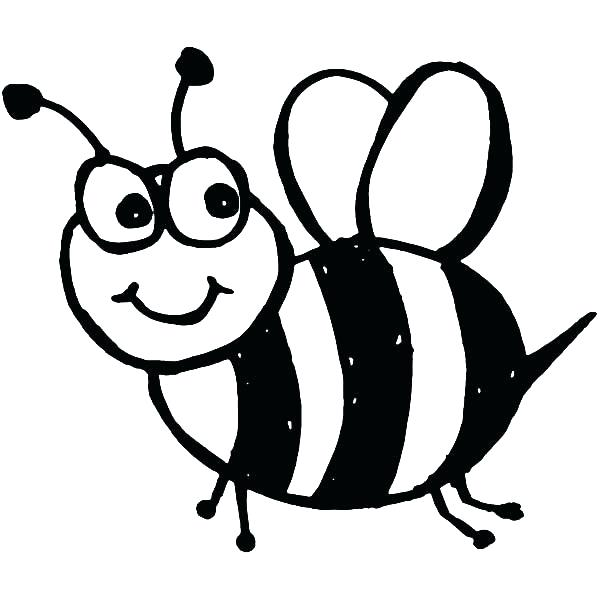
\includegraphics[width=.25\linewidth]{images/vcelka.jpg}
\end{center}
\caption*{Včelička \cite{vcelicka}}
\end{figure}

\label{chap:conclusion}
\addcontentsline{toc}{chapter}{\nameref{chap:conclusion}}
\printbibliography
\end{document}
